\chapter{구속계와 해밀턴 운동}

\lectureoverview{두 가지 구속계는 라그랑주 역학이 왜 그토록 효과적인지를 보여 준다. 적절한 좌표를 선택하면 구속력을 명시적으로 계산하지 않고도 운동 방정식과 보존 법칙을 얻을 수 있다. 이어지는 같은 예제들은 해밀턴 역학으로 나아간다. 해밀턴 역학에서는 좌표와 운동량이 위상공간을 이루고, 조화 진동자는 강체 회전으로 나타나며, 2계 오일러--라그랑주 방정식은 해밀턴의 두 1계 방정식으로 대체된다.}

\section{역학 문제를 푼다는 것의 의미}

라그랑주 방법의 직접적인 목적은 실용적인 데 있다. 바닥 위를 미끄러지는 쐐기와 이중 진자는 모두 뉴턴 법칙으로 다룰 수 있지만, 미지의 접촉력과 장력을 일일이 계산하다 보면 금세 번거로워진다. 라그랑주 역학의 규칙을 알고 나면 같은 문제를 다음과 같이 단계적으로 다룰 수 있다:
\begin{enumerate}
  \item 순간적인 배치를 나타내는 독립 좌표를 선택한다;
  \item 그 좌표로 운동 에너지와 퍼텐셜 에너지를 표현한다;
  \item \(L=T-V\)를 구성하고 오일러--라그랑주 방정식을 적용한다.
\end{enumerate}

현재의 목적에서는 운동 방정식을 올바르게 세웠을 때 이미 문제를 \emph{풀었다}고 본다. 닫힌 형태의 궤적을 구하고 싶을 수도 있지만, 그것은 별개의 문제다. 역학적 설정을 마치고 나면 비선형 미분 방정식은 수치적으로 적분할 수 있다. 어려운 부분은 흔히 적분이 아니라, 불필요한 미지의 힘을 도입하지 않고 구속 조건을 반영하는 변수를 찾는 일이다.

\section{움직이는 쐐기 위를 미끄러지는 입자}

질량이 \(M\)인 쐐기가 마찰 없이 수평면을 따라 미끄러지도록 구속되어 있다고 하자. 질량이 \(m\)인 점입자는 경사면 위에 머물도록 구속되어 있다. 자유도는 두 개다. 하나는 쐐기의 위치를, 다른 하나는 쐐기 위에서 입자가 있는 위치를 나타낸다.

다음과 같이 두자.
\begin{equation}
  \begin{aligned}
    X&=\text{horizontal position of the wedge corner},\\
    x&=\text{horizontal displacement of the particle}\\[-0.2em]
     &\phantom{={}}\text{from that corner}.
  \end{aligned}
  \label{eq:l6-wedge-coordinates}
\end{equation}
따라서 입자의 절대 수평 좌표는 \(X+x\)이다. 좌표 선택은 하나로 정해져 있지 않다. 경사면을 따라 잰 거리나 입자의 절대 수평 좌표를 사용할 수도 있다. 같은 배치를 나타내는 비중복 좌표 쌍이라면 무엇이든 쓸 수 있지만, 어떤 쌍은 다른 쌍보다 계의 구조를 더 분명하게 드러낸다.

경사각 \(\beta\)이 고정되어 있으면 수직 변위 \(y\)는 독립적인 좌표가 아니다:
\begin{equation}
  y=x\tan\beta,
  \qquad
  \dot y=\dot x\tan\beta.
  \label{eq:l6-wedge-constraint}
\end{equation}
이제 \(\beta=45^\circ\)인 경우로 한정하면 \(y=x\)이고
\(\dot y=\dot x\)이다.  이 단순화는 예제의 요점을 바꾸지 않으면서 삼각함수 인자를 없앤다.

\begin{figure}[htbp]
  \centering
  \includegraphics[width=0.84\textwidth]{lecture_06_figure_06.png}
  \caption{\(45^\circ\) 예제에서 사용한 움직이는 쐐기와 구속된 입자, 수평 및 수직 속도 성분.}
  \lectureframe{00:10:25}
\end{figure}

쐐기의 운동 에너지는 다음과 같다.
\begin{equation}
  T_{M}=\frac{M}{2}\dot X^2.
  \label{eq:l6-wedge-kinetic}
\end{equation}
입자의 수평 속도는 \(\dot X+\dot x\)이고 수직 속도는 \(\dot x\)이다. 따라서 입자의 운동 에너지는
\begin{equation}
  T_m=\frac{m}{2}\left[(\dot X+\dot x)^2+\dot x^2\right].
  \label{eq:l6-particle-kinetic}
\end{equation}
중력 퍼텐셜의 영점을 \(x=0\)에 두면 \(V=mgx\)이다. 그러므로
\begin{equation}
  L=\frac{M}{2}\dot X^2
    +\frac{m}{2}\left[(\dot X+\dot x)^2+\dot x^2\right]
    -mgx.
  \label{eq:l6-wedge-lagrangian}
\end{equation}

\begin{figure}[htbp]
  \centering
  \includegraphics[width=0.86\textwidth]{lecture_06_figure_07.png}
  \caption{쐐기의 기하와 \(V=mgx\), 그리고 칠판에 정리한 두 운동 에너지 항.}
  \lectureframe{00:14:15}
\end{figure}

\subsection{정준운동량은 라그랑지안으로 정의된다}

정준운동량은 입자 속도 하나를 보고 짐작하는 것이 아니라 라그랑지안으로 정의한다:
\begin{align}
  p_X&=\frac{\partial L}{\partial\dot X}
      =M\dot X+m(\dot X+\dot x),
      \label{eq:l6-wedge-pX}\\
  p_x&=\frac{\partial L}{\partial\dot x}
      =m(\dot X+\dot x)+m\dot x.
      \label{eq:l6-wedge-px}
\end{align}
첫 번째 식은 보통의 전체 수평 운동량이다. 쐐기가 \(M\dot X\)만큼 기여하고, 입자가 \(m(\dot X+\dot x)\)만큼 기여한다. 이 운동량은 여기서 좌표 \(X\)에 켤레인 운동량으로 나타난다.

\begin{figure}[htbp]
  \centering
  \includegraphics[width=0.86\textwidth]{lecture_06_figure_08.png}
  \caption{쐐기 좌표 \(X\)와 입자의 상대 좌표 \(x\)에 켤레인 정준운동량.}
  \lectureframe{00:18:05}
\end{figure}

라그랑지안은 \(X\)에 명시적으로 의존하지 않는다. 장치 전체의 수평 병진 변환은 다음과 같이 작용한다.
\begin{equation}
  \delta X=\epsilon,
  \qquad
  \delta x=0.
  \label{eq:l6-wedge-translation}
\end{equation}
따라서 일반적인 무한소 대칭 규칙
\begin{equation}
  \delta q_i=\epsilon f_i(q),
  \qquad
  Q=\sum_i p_i f_i
  \label{eq:l6-noether-rule}
\end{equation}
에 따라 \(Q=p_X\)이다. 달리 말해 \(X\)는 순환 좌표이며,
\begin{equation}
  \dot p_X=\frac{\partial L}{\partial X}=0.
  \label{eq:l6-wedge-conservation}
\end{equation}

이에 대응하는 수직 병진 대칭은 없다. 쐐기는 수직으로 움직일 수 없고, 입자의 높이가 바뀌면 중력 퍼텐셜도 바뀐다. 수평 운동량은 보존되지만, 이 구속된 계의 수직 운동량은 보존되지 않는다.

상대 좌표에 대한 오일러--라그랑주 방정식은 다음과 같다.
\begin{equation}
  \dot p_x=\frac{\partial L}{\partial x}=-mg.
  \label{eq:l6-wedge-force}
\end{equation}
이 식은 칠판에서 부호를 바로잡아야 했다. 믿을 수 있는 방법은 \(L=T-V\)에서 시작하는 것이다. \(V=mgx\)이므로 라그랑지안의 미분은 \(-mg\)이다. \(x\)를 수평 변위로 도입했더라도 그 방정식에서 중력이 사라지는 것은 아니다. 구속 조건이 그 수평 변위를 수직 높이 \(y=x\)와 연결하기 때문이다.

수직항력이나 반작용력은 등장하지 않는다. 이런 힘은 구속 조건을 유지하는 데 필요한 만큼 작용한다. 뉴턴 방법에서는 이 힘들을 도입해 가속도와 함께 구해야 하지만, 일반화 좌표를 사용하면 그럴 필요가 없다.

\section{이중 진자와 좌표 선택의 묘미}

이제 질량이 각각 단위 질량인 두 물체를 길이가 단위 길이인 질량 없는 막대 두 개에 매달아 보자.  첫 번째 막대는 아래쪽 수직선과 \(\theta\)의 각을 이룬다.  두 번째 자유도에는 두 가지 선택지가 있다. 두 번째 절대각 \(\phi\)를 사용하거나, 두 막대 사이의 상대각 \(\alpha\)을 사용할 수 있다.

상대각을 선택하는 편이 계의 구조를 더 잘 드러낸다. 잠시 중력을 끄자. 장치 전체를 강체 회전시키면 절대 방향은 바뀌지만 막대 사이의 각도는 변하지 않는다:
\begin{equation}
  \theta\longrightarrow\theta+\epsilon,
  \qquad
  \alpha\longrightarrow\alpha.
  \label{eq:l6-double-rotation}
\end{equation}
이 좌표를 선택하면 회전 대칭은 하나의 좌표에만 작용한다. 그렇다고 다른 좌표계가 틀린 것은 아니다. 이 선택에서는 대칭과 그에 따른 보존량을 더 쉽게 알아볼 수 있다.

\begin{figure}[htbp]
  \centering
  \includegraphics[width=0.76\textwidth]{lecture_06_figure_09.png}
  \caption{첫 번째 절대각이 \(\theta\)이고 두 번째 막대의 각도가 첫 번째 막대에 대한 상대각 \(\alpha\)인 이중 진자.}
  \lectureframe{00:29:20}
\end{figure}

운동 에너지를 구할 때는 계산을 위한 보조 수단으로 데카르트 좌표를 사용하자. 수직 좌표를 아래쪽 방향으로 재면 첫 번째 추의 위치는
\begin{equation}
  x_1=\sin\theta,
  \qquad
  y_1=\cos\theta,
  \label{eq:l6-bob-one-position}
\end{equation}
이므로
\begin{equation}
  \dot x_1=\dot\theta\cos\theta,
  \qquad
  \dot y_1=-\dot\theta\sin\theta,
  \qquad
  \dot x_1^2+\dot y_1^2=\dot\theta^2.
  \label{eq:l6-bob-one-velocity}
\end{equation}
두 번째 추의 위치는
\begin{align}
  x_2&=\sin\theta+\sin(\theta+\alpha),\\
  y_2&=\cos\theta+\cos(\theta+\alpha),
  \label{eq:l6-bob-two-position}
\end{align}
따라서 예를 들어
\begin{equation}
  \dot x_2=\dot\theta\cos\theta
  +(\dot\theta+\dot\alpha)\cos(\theta+\alpha),
  \label{eq:l6-bob-two-xvelocity}
\end{equation}
이며, \(\dot y_2\)에도 같은 방식의 식이 성립한다.

\begin{figure}[htbp]
  \centering
  \includegraphics[width=0.88\textwidth]{lecture_06_figure_10.png}
  \caption{두 추가 위치를 나타내는 보조 데카르트 좌표. 이 좌표는 속도를 계산하는 데 쓰이며 추가 자유도로 도입한 것은 아니다.}
  \lectureframe{00:35:25}
\end{figure}

두 운동 에너지를 더하면 다음과 같이 일관된 결과를 얻는다. 교차항은 다음 항등식에서 나온다.
\begin{equation*}
  \cos A\cos B+\sin A\sin B=\cos(A-B).
\end{equation*}
\begin{equation}
  T=\dot\theta^2
    +\frac12(\dot\theta+\dot\alpha)^2
    +\dot\theta(\dot\theta+\dot\alpha)\cos\alpha.
  \label{eq:l6-double-kinetic}
\end{equation}

\begin{classroomqa}
  \audiencequestion{이 식에는 두 추의 운동 에너지가 이미 모두 포함되어 있나요? 혹시 2분의 1 계수가 빠진 것은 아닌가요?
  \lecturetimestamp{00:38:06--00:38:27}}
  \lecturerresponse{두 추의 운동 에너지가 모두 포함되어 있습니다. 이 식은
  \(\tfrac12(\dot x_1^2+\dot y_1^2+\dot x_2^2+\dot y_2^2)\)에서 나옵니다.
  두 기여가 같아서 합하면 첫 번째 항 \(\dot\theta^2\)이 됩니다. 빠진 계수는 없습니다.}
\end{classroomqa}

중력이 없으면 \(L=T\)에는 \(\theta\)가 명시적으로 나타나지 않는다. 따라서
\begin{equation}
  \dot p_\theta=\frac{\partial L}{\partial\theta}=0,
  \label{eq:l6-double-angular-conservation}
\end{equation}
이고, \(p_\theta\)는 전체 각운동량이다. \(\theta\)가 나타나지 않는다는 말의 정확한 의미에 주목하자. \(\dot\theta\)는 분명히 나타나지만, 미분되지 않은 좌표 자체는 나타나지 않는다.

중력을 다시 켜면 전역 회전 대칭이 깨진다. 앞서 정한 수직 좌표의 아래쪽 방향 규약에 따라 영점을 편리하게 정하면
\begin{equation}
  V=-g(y_1+y_2)
   =-g\left[2\cos\theta+\cos(\theta+\alpha)\right].
  \label{eq:l6-double-potential}
\end{equation}
상수를 더해도 결과는 달라지지 않는다. 중요한 점은 이제 \(\theta\)가 식에 명시적으로 나타나므로 그에 켤레인 운동량이 더는 보존되지 않는다는 것이다. 라그랑지안이 시간에 명시적으로 의존하지 않으므로 에너지는 계속 보존된다.

\begin{classroomqa}
  \audiencequestion{칠판의
  \(\dot\theta-\dot\alpha\)는
  \(\dot\theta+\dot\alpha\)이어야 하나요?
  \lecturetimestamp{00:43:00--00:43:54}}
  \lecturerresponse{여기서 사용한 방향 규약에서는 플러스 부호가 맞습니다. 이는 식 ~\eqref{eq:l6-bob-two-position}의 규약이며 운동 에너지 식 ~\eqref{eq:l6-double-kinetic}에도 그대로 적용됩니다. 양의 방향을 \(\alpha\)의 정의에서 반대로 정하면 관련 부호도 바뀌지만, 그 경우에는 모든 항에서 일관되게 바꾸어야 합니다. 칠판에서는 두 규약이 뒤섞였습니다.}
\end{classroomqa}

\begin{figure}[htbp]
  \centering
  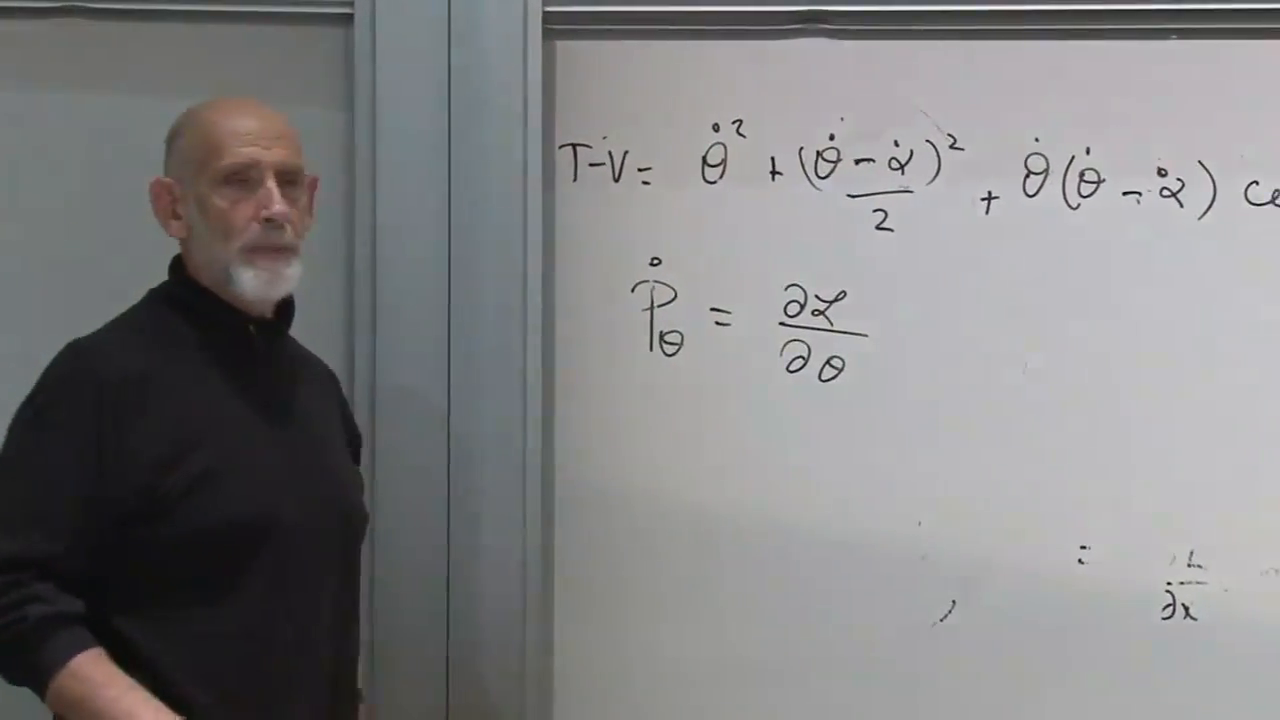
\includegraphics[width=0.84\textwidth]{lecture_06_figure_02.png}
  \caption{중력이 없는 이중 진자 계산과 \(\dot p_\theta=\partial L/\partial\theta\). 위쪽 칠판 식은 질문에서 다룬 부호 불일치가 있는 국소 표기를 그대로 보여 주며, 정규화된 식은 식 ~\eqref{eq:l6-double-kinetic}이다.}
  \lectureframe{00:45:50}
\end{figure}

\(T\)와 \(V\)를 알고 나면 나머지 방정식은 미분하여 얻을 수 있다. 막대의 장력과 고정된 길이를 유지하는 힘은 이번에도 좌표 선택에 흡수되어 나타나지 않는다.

\subsection{보존이 의미하는 것과 의미하지 않는 것}

\begin{classroomqa}
  \audiencequestion{방정식만 보고 이중 진자가 카오스적인지 직접 알 수 있나요?
  \lecturetimestamp{00:44:57--00:45:25}}
  \lecturerresponse{대개는 간단히 살펴보는 것만으로는 알기 어렵습니다. 매개변수나 에너지가 변하면 계의 거동이 규칙적 운동에서 카오스적 운동으로 바뀔 수 있습니다. 이 주제를 다루려면 방정식의 겉모습보다 더 많은 구조가 필요하며, 뒤에서 살펴보겠습니다.}
\end{classroomqa}

\begin{classroomqa}
  \audiencequestion{보존계에서는 모든 \(\dot p_i\)가
  영인가?
  \lecturetimestamp{00:45:25--00:46:24}}
  \lecturerresponse{아니다.  일반적인 방정식은
  \(\dot p_i=\partial L/\partial q_i\)이다.  \(q_i\)가 순환좌표일 때에만
  이 값은 영이 된다.  순환좌표는 다른 좌표들은 고정한 채 한 좌표만 이동시키는 대칭성이 주어진 특별히 단순한 경우다.}
\end{classroomqa}

목표가 수치적 시간 발전뿐이라면 불편한 좌표계를 써도 된다. 단지 방정식이 길어질 뿐이다. 좌표계를 잘 선택했을 때 얻는 이점은 개념적인 데 있다. 방정식을 풀기 전부터 보존 운동량을 알아볼 수 있다.

\begin{classroomqa}
  \audiencequestion{중력이 없으면 이중 진자는 하나의 자유 진자만큼
  단순하게 운동하는가?
  \lecturetimestamp{00:47:02--00:47:35}}
  \lecturerresponse{하나의 자유 로터는 각운동량 하나가 운동을 결정하므로
  등속 회전한다.  이중 진자는 전체 각운동량을 보존하면서도
  매우 복잡한 상대 운동을 할 수 있다.  처음에 두 각속도가 모두
  영이면 정지 상태를 유지하고, 그렇지 않으면 두 부분이 서로
  상호작용한다.}
\end{classroomqa}

\begin{classroomqa}
  \audiencequestion{중력이 없을 때 \(\dot\theta\)와 \(\dot\alpha\)는 각각 일정한가요?
  \lecturetimestamp{00:47:36--00:52:42}}
  \lecturerresponse{아닙니다. 보존 법칙은 \(\dot p_\theta=0\)라는 뜻이지, \(\ddot\theta=0\) 또는 \(\ddot\alpha=0\)라는 뜻은 아닙니다. \(p_\theta=\partial L/\partial\dot\theta\)의 식에는 두 각속도가 모두 들어가며 \(\alpha\)에도 의존합니다. 막대는 토크를 전달하여 두 추가 각운동량과 에너지를 주고받게 합니다. 이는 스프링으로 연결된 두 질점의 경우와 비슷합니다. 전체 운동량과 질량중심 속도는 일정하지만, 각 질점의 속도는 진동합니다. 회전에 대응하는 보존량은 두 각 가운데 어느 하나가 아니라 특정한 집단적 조합입니다.}
\end{classroomqa}

\begin{classroomqa}
  \audiencequestion{각운동량을 주고받게 하는 힘은 막대를 통해
  전달되는가?
  \lecturetimestamp{00:52:43--00:53:34}}
  \lecturerresponse{그렇다.  막대를 따라 전달되는 힘은 다른 운동의
  회전축을 지나지 않을 수 있으므로 토크를 가할 수 있다.  토크는
  힘이 일으키는 회전 경향일 뿐이며, 여기서는 각 부분에 영이 아닌
  각가속도를 만든다.}
\end{classroomqa}

\section{세 번째 정식화로서의 해밀턴 역학}

해밀토니안은 에너지이지만, 그것은 해밀토니안의 첫 번째 의미일 뿐이다. 해밀토니안은 역학의 세 번째 정식화의 토대이기도 하다. 뉴턴 방정식은 힘과 가속도를 사용한다. 정지 작용 원리는 오일러--라그랑주 방정식을 준다. 정칙계에서 해밀턴 역학은 후자와 동등하지만, 사용하는 변수와 기하학적 구조는 다르게 보인다.

\(q_i\)와 \(\dot q_i\) 대신 \(q_i\)와 그에 켤레인 운동량 \(p_i\)를 사용하자. 자유도가 \(n\)개인 계의 상태는 어느 표현에서든 \(2n\)개의 수로 나타낸다. 즉 위치와 속도 또는 위치와 운동량으로 나타낼 수 있다. 둘 사이의 연결은 다음과 같다.
\begin{equation}
  p_i=\frac{\partial L}{\partial\dot q_i}.
  \label{eq:l6-legendre-map}
\end{equation}
이 관계를 속도에 대해 풀 수 있다면
\(\dot q_i(q,p)\)해밀토니안을 다음과 같이 정의한다.
\begin{equation}
  H(q,p)=\sum_i p_i\dot q_i-L(q,\dot q).
  \label{eq:l6-hamiltonian-definition}
\end{equation}
그러면 우변의 속도를 없애고 \(q\)와 \(p\)만으로 표현할 수 있다. 이 가역성이 정칙 르장드르 변환의 가정이다. 특이 라그랑지안에는 더 일반적인 구속 조건 이론이 필요하므로, 이 기초적인 구성으로는 다루지 않는다.

\subsection{미적분에 앞서 되돌릴 수 있음 살펴보기}

화살표로 연결된 유한한 추상 상태 집합을 떠올려 보자. 결정론적 규칙이라도 이전 상태 둘이 하나의 나중 상태로 흘러들어 가면 되돌릴 수 없을 수 있다. 미래는 하나로 정해지지만 과거는 유일하지 않다. 화살표를 모두 뒤집으면 반대 문제가 생긴다. 하나의 상태에서 여러 미래가 갈라져 나온다. 첫 번째 그림에서는 화살표가 모이고, 두 번째 그림에서는 갈라진다.

\begin{figure}[htbp]
  \centering
  \includegraphics[width=0.86\textwidth]{lecture_06_figure_11.png}
  \caption{되돌릴 수 있는 순환과 허용되지 않는 수렴 및 발산을 대비하기 위한 추상 상태 사상.}
  \lectureframe{00:56:20}
\end{figure}

해밀턴 흐름은 이 진술을 연속적인 경우로 확장해 준다. 위상공간의 점들로 이루어진 구름은 움직이고 변형될 수 있지만, 상태 사이의 차이를 없애는 흡인점이나 하나의 상태에서 여러 미래를 만들어 내는 발산점은 생길 수 없다. 증명은 뒤로 미루고, 지금은 이 도식들을 통해 기하학적 관점을 살펴보자.

\begin{classroomqa}
  \audiencequestion{추상 상태 도식을 중력장에서 움직이는 물체로 해석해야 하나요?
  \lecturetimestamp{00:58:02--00:58:35}}
  \lecturerresponse{아닙니다. 점은 그저 추상적인 상태이고 화살표는 상태를 바꾸는 규칙을 나타냅니다. 이 그림에는 공간적 의미나 중력의 의미가 부여되어 있지 않습니다.}
\end{classroomqa}

\begin{classroomqa}
  \audiencequestion{허용되지 않는 수렴 상태 사상은 블랙홀과 어떻게 구별하나요?
  \lecturetimestamp{00:58:40--00:59:28}}
  \lecturerresponse{쉽지 않고, 미묘한 문제입니다. 타당한 질문이지만, 올바르게 답하려면 전체 상태와 그 양자 중력적 시간 발전을 세심하게 살펴야 합니다. 기초적인 도식만으로는 결론을 내릴 수 없습니다.}
\end{classroomqa}

\section{위상공간에 맞춘 진동자}

일반 방정식을 유도하기 전에, 위상공간에 맞게 의도적으로 표현한 조화 진동자를 살펴보자:
\begin{equation}
  L=\frac{1}{2\omega}\dot q^2-\frac{\omega}{2}q^2.
  \label{eq:l6-rescaled-lagrangian}
\end{equation}
켤레 운동량은 다음과 같다.
\begin{equation}
  p=\frac{\partial L}{\partial\dot q}=\frac{\dot q}{\omega},
  \qquad
  \dot q=\omega p.
  \label{eq:l6-rescaled-momentum}
\end{equation}
이를 식 ~\eqref{eq:l6-hamiltonian-definition}에 대입하면
\begin{align}
  H&=p\dot q-L\\
   &=\omega p^2-\frac{\omega p^2}{2}+\frac{\omega q^2}{2}
    =\frac{\omega}{2}(p^2+q^2).
  \label{eq:l6-oscillator-hamiltonian}
\end{align}

\begin{figure}[htbp]
  \centering
  \includegraphics[width=0.86\textwidth]{lecture_06_figure_12.png}
  \caption{위상공간에 맞춘 진동자의 르장드르 변환과 대칭적인 해밀토니안 \(H=\tfrac{\omega}{2}(p^2+q^2)\).}
  \lectureframe{01:08:20}
\end{figure}

\(q\)와 \(p\)로 이루어진 공간이 위상공간이다. 자유도가 하나이면 2차원 평면이고, 자유도가 둘이면 4차원 위상공간이다. 진동자의 에너지가 일정하면
\begin{equation}
  p^2+q^2=\frac{2H}{\omega},
  \label{eq:l6-energy-circle}
\end{equation}
궤적은 원 위에 머문다. 에너지 보존에 따라 운동은 그 원 가운데 하나에 제한된다.

\begin{figure}[htbp]
  \centering
  \includegraphics[width=0.82\textwidth]{lecture_06_figure_13.png}
  \caption{진동자의 위상평면에서 에너지가 일정한 동심원. 가로축은 \(q\), 세로축은 \(p\)이다.}
  \lectureframe{01:13:20}
\end{figure}

\section{해밀턴 방정식 유도}

유도 과정은 여러 변수의 함수에 대한 전미분을 다루는 연습이다. \(F(q,p)\)에 대해
\begin{equation}
  \delta F=\sum_i\left(
  \frac{\partial F}{\partial q_i}\delta q_i
  +\frac{\partial F}{\partial p_i}\delta p_i\right).
  \label{eq:l6-total-differential}
\end{equation}
계수는 어느 방향으로든 읽을 수 있다. \(\delta q_i\)의 계수는 \(\partial F/\partial q_i\)이고, \(\delta p_i\)의 계수는 \(\partial F/\partial p_i\)이다.

이제 \(H\)의 정의식을 변분하자:
\begin{align}
  \delta H
  &=\sum_i\left(\dot q_i\,\delta p_i
       +p_i\,\delta\dot q_i\right)-\delta L\\
  &=\sum_i\left(\dot q_i\,\delta p_i
       +p_i\,\delta\dot q_i
       -\frac{\partial L}{\partial q_i}\delta q_i
       -\frac{\partial L}{\partial\dot q_i}\delta\dot q_i\right).
  \label{eq:l6-vary-hamiltonian}
\end{align}
\(\partial L/\partial\dot q_i=p_i\)이므로 두 \(\delta\dot q_i\)항이 상쇄된다. 오일러--라그랑주 방정식에 따라 \(\partial L/\partial q_i=\dot p_i\)이므로, 남는 식은
\begin{equation}
  \delta H=\sum_i\left(\dot q_i\,\delta p_i
                     -\dot p_i\,\delta q_i\right).
  \label{eq:l6-reduced-variation}
\end{equation}

\begin{figure}[htbp]
  \centering
  \includegraphics[width=0.86\textwidth]{lecture_06_figure_14.png}
  \caption{\(\delta H\)를 전개한 곱의 미분식. \(p_i\,\delta\dot q_i\)항이 상쇄되기 전의 식이다.}
  \lectureframe{01:18:40}
\end{figure}

식 ~\eqref{eq:l6-reduced-variation}을 식 ~\eqref{eq:l6-total-differential}의 일반적인 전미분과 비교하면, 서로 독립인 계수로부터 해밀턴 방정식을 얻는다:
\begin{equation}
  \boxed{
  \dot q_i=\frac{\partial H}{\partial p_i},
  \qquad
  \dot p_i=-\frac{\partial H}{\partial q_i}.}
  \label{eq:l6-hamilton-equations}
\end{equation}

\begin{figure}[htbp]
  \centering
  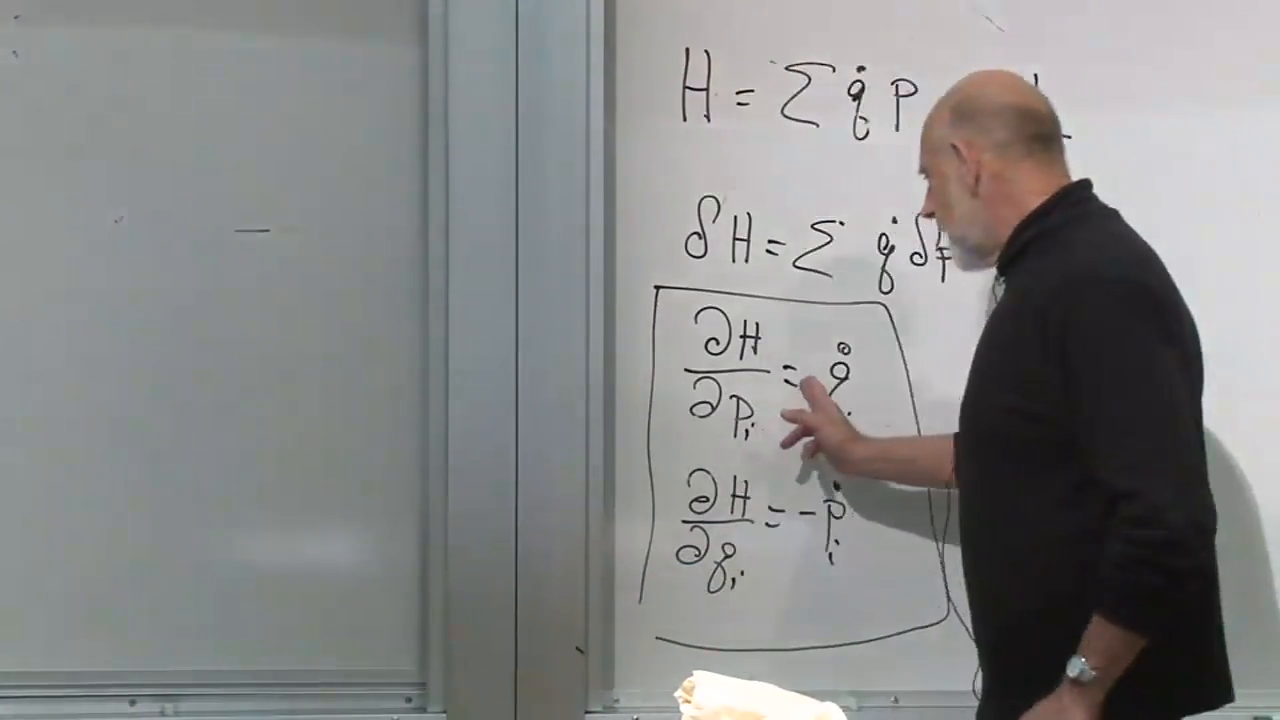
\includegraphics[width=0.78\textwidth]{lecture_06_figure_03.png}
  \caption{해밀토니안의 정의와 그 변분, 그리고 상자로 표시한 정준 방정식.}
  \lectureframe{01:22:18}
\end{figure}

\(n\)개의 좌표에 대해 이 식들은 1계 방정식 \(2n\)개를 이룬다. 반면 오일러--라그랑주 정식화는 2계 방정식 \(n\)개를 준다. 필요한 초기 조건의 양과 물리적 내용은 동일하다.

\section{진동자 운동은 강체 회전이다}

식 ~\eqref{eq:l6-hamilton-equations}을 식 ~\eqref{eq:l6-oscillator-hamiltonian}에 적용하면
\begin{equation}
  \dot q=\omega p,
  \qquad
  \dot p=-\omega q.
  \label{eq:l6-oscillator-first-order}
\end{equation}첫 번째 방정식을 미분하고 두 번째 방정식을 사용하면
\begin{equation}
  \ddot q=\omega\dot p=-\omega^2q.
  \label{eq:l6-oscillator-second-order}
\end{equation}따라서 두 1계 방정식은 운동량의 정의와 함께 보통의 2계 진동자 방정식을 정확히 재현한다.

위상공간에서 \((q,p)\)에 해당하는 속도 벡터는 \((\dot q,\dot p)=(\omega p,-\omega q)\)이며, 에너지 원에 접한다. 모든 반지름은 같은 각속도 \(\omega\)로 회전한다. 평면 전체를 강체 바람개비나 압축되지 않는 가상 유체로 생각할 수 있다. 점들은 순환하지만, 흡인점으로 모이거나 발산점에서 퍼져 나가지는 않는다.

\begin{figure}[htbp]
  \centering
  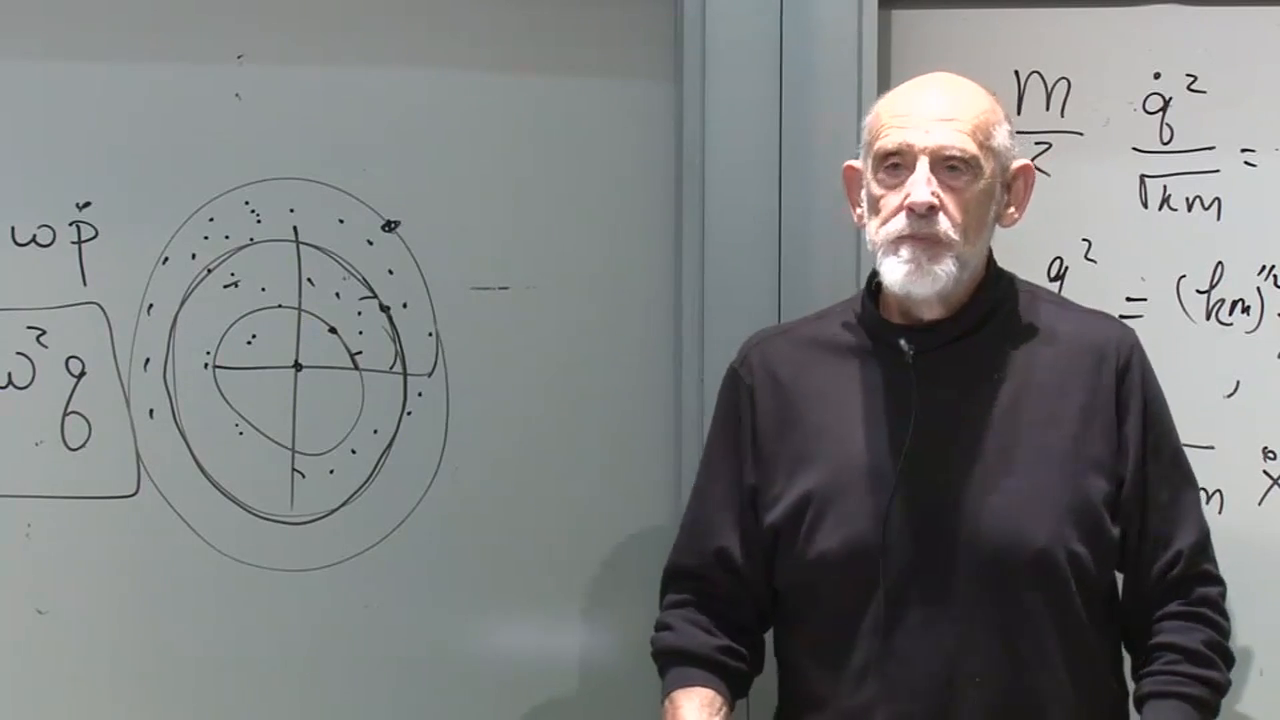
\includegraphics[width=0.86\textwidth]{lecture_06_figure_04.png}
  \caption{위상공간의 여러 궤적에 분포한 초기점들의 구름. 해밀턴 시간 발전은 구름을 선호되는 한 상태로 붕괴시키지 않고 구름 전체를 움직인다.}
  \lectureframe{01:39:27}
\end{figure}

\begin{figure}[htbp]
  \centering
  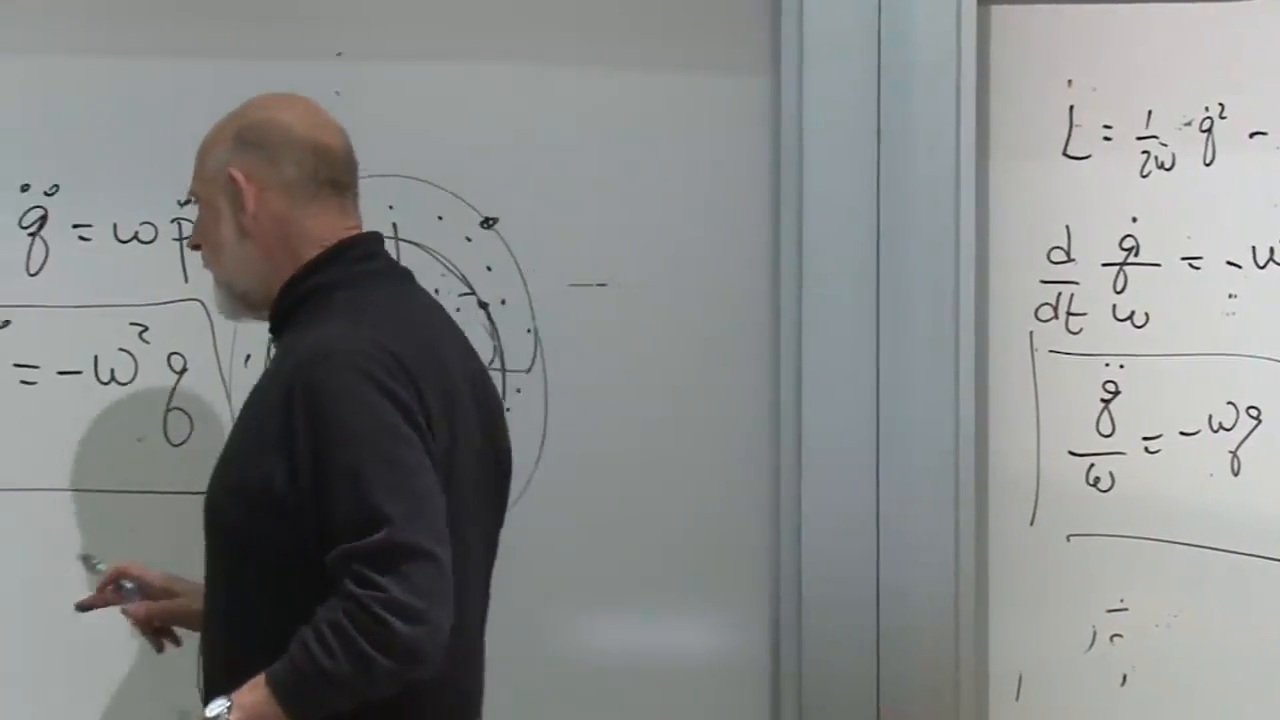
\includegraphics[width=0.90\textwidth]{lecture_06_figure_05.png}
  \caption{진동자의 위상도와 그에 동등한 오일러--라그랑주 방정식 \(\ddot q/\omega=-\omega q\).}
  \lectureframe{01:42:10}
\end{figure}

다음 단계에서는 유체 비유를 정리로 바꾸어, 해밀턴 흐름에는 국소적인 수렴이나 발산이 없음을 보일 것이다. 이 결과는 연속 역학을 강의 초반에 살펴본 가역 상태 사상과 다시 연결해 준다.

\section{좌표 선택의 의미를 드러내는 질문}

\begin{classroomqa}
  \audiencequestion{속도를 \(q\)와 \(p\)로 나타낼 수 있다는 가정은 정리인가요, 아니면 물리계의 경험적 성질인가요?
  \lecturetimestamp{01:29:08--01:29:45}}
  \lecturerresponse{이 기초적인 전개에서는 경험적으로 성립하는 규칙성으로 다루며, 양자역학에서 더 깊은 동기를 찾을 수 있습니다. 더 정확히 말하면 식 ~\eqref{eq:l6-legendre-map}의 속도에 대한 야코비안이 비특이행렬이어야 합니다. 현대 역학에는 중요한 특이 라그랑지안도 있으며, 특히 구속계와 게이지 계에서 나타납니다. 이런 계를 해밀턴 형식으로 다루려면 추가적인 구속 조건 형식이 필요합니다.}
\end{classroomqa}

단위에 관한 의문을 살펴보면 진동자를 식 ~\eqref{eq:l6-rescaled-lagrangian}의 익숙하지 않은 형태로 쓴 이유가 분명해진다. 먼저 보통 좌표 \(x\)에서 시작하자:
\begin{equation}
  L=\frac{m}{2}\dot x^2-\frac{k}{2}x^2,
  \qquad
  \omega=\sqrt{\frac{k}{m}}.
  \label{eq:l6-ordinary-oscillator}
\end{equation}
다음과 같이 두자.
\begin{equation}
  q=(km)^{1/4}x.
  \label{eq:l6-oscillator-rescaling}
\end{equation}
그러면 \(q^2=\sqrt{km}\,x^2\)이고
\(\dot q^2=\sqrt{km}\,\dot x^2\)이므로, 식 ~\eqref{eq:l6-ordinary-oscillator}은 정확히 식 ~\eqref{eq:l6-rescaled-lagrangian}으로 바뀐다. 새로운 \(q\)는 맞춤형 일반화 좌표이지 길이가 아니며, 그 켤레 \(p\)도 보통의 역학적 운동량 \(p_x=m\dot x\)가 아니다.

\begin{figure}[htbp]
  \centering
  \includegraphics[width=0.86\textwidth]{lecture_06_figure_15.png}
  \caption{보통의 진동자 좌표 \(x\)에서 맞춤형 좌표 \(q=(km)^{1/4}x\)로의 차원 재조정.}
  \lectureframe{01:36:10}
\end{figure}

\begin{classroomqa}
  \audiencequestion{\(\omega p=\dot q\)은 어떻게 차원적으로 일관되며, 왜 이 변수들을 선택했나요?
  \lecturetimestamp{01:29:46--01:39:22}}
  \lecturerresponse{\(q\)의 차원이 길이일 필요는 없고, 그 켤레 \(p\)의 차원도 \(m\dot x\)와 같을 필요는 없습니다. 식 ~\eqref{eq:l6-oscillator-rescaling}의 재조정은 라그랑지안의 차원을 보존하며 \(q\)와 \(p\)가 \(H\)에 대칭적으로 들어가게 합니다. 원래 변수로 쓰면
  \[
    H=\frac{p_x^2}{2m}+\frac{kx^2}{2},
  \]
따라서 \((x,p_x)\) 평면에서 에너지가 일정한 곡선은 타원입니다. 맞춤형 \((q,p)\) 평면에서는 원이 됩니다. 이러한 대칭이 드러나도록 재조정을 선택했습니다.}
\end{classroomqa}

\begin{classroomqa}
  \audiencequestion{\(2n\)개의 1계 해밀턴 방정식이 \(n\)개의 2계 라그랑주 방정식과 어떻게 동등할 수 있나요?
  \lecturetimestamp{01:39:24--01:42:30}}
  \lecturerresponse{진동자의 경우 \(\dot q=\omega p\)를 미분하고 \(\dot p=-\omega q\)를 대입하면 두 식은 \(\ddot q=-\omega^2q\)가 됩니다. 라그랑지안에서 바로 출발하면
  \[
    \frac{d}{dt}\left(\frac{\dot q}{\omega}\right)
      =-\omega q,
  \]
같은 2계 방정식을 얻습니다. 해밀턴 방정식 하나는 속도로부터 운동량을 정의하고, 다른 하나는 그 운동량의 시간 변화를 나타낸다고 볼 수 있습니다.}
\end{classroomqa}

\section{위상공간과 퍼텐셜 에너지가 중요한 이유}

\begin{classroomqa}
  \audiencequestion{해밀토니안의 유용성이 위상공간이 배치공간보다 더 나은 기하학적 표현임을 뜻하나요?
  \lecturetimestamp{01:42:33--01:44:38}}
  \lecturerresponse{두 공간은 서로 다른 목적에 쓰입니다. 위상공간에서는 순환 운동과 에너지 일정면, 그리고 수렴이나 발산의 부재가 특히 분명하게 드러납니다. 다른 문제에서는 배치공간이 더 유용할 수 있습니다. \(H\)를 강조하는 더 깊은 이유는 이것이 양자역학에서 핵심적이고 더 직관적인 대상이 되기 때문입니다. 양자역학은 이 역학 강의가 나아가는 현대 물리학의 주제 가운데 하나입니다.}
\end{classroomqa}

\begin{classroomqa}
  \audiencequestion{퍼텐셜 에너지를 힘의 적분으로 보아야 하나요?
  \lecturetimestamp{01:44:40--01:45:45}}
  \lecturerresponse{보존력이라면 상수항과 적절한 부호를 고려해 그 말이 맞습니다. 하지만 퍼텐셜을 기본량으로 두고 그로부터 일반화 힘을 구하는 편이 더 유용합니다:
  \[
    F_i=-\frac{\partial V}{\partial q_i}.
  \]
이는 \(\dot p_i=\partial L/\partial q_i\)에 나타나는 바로 그 항이며, 이때 \(L=T-V\)이고 운동 에너지는 \(q_i\)에 명시적으로 의존하지 않습니다.}
\end{classroomqa}

\begin{classroomqa}
  \audiencequestion{현대 물리학으로 이어지는 이 경로는 어떤 최전선의 문제를 밝히려는 것인가요?
  \lecturetimestamp{01:45:46--01:47:47}}
  \lecturerresponse{이 경로는 양자 중력과 우주론, 힉스 부문과 중성미자를 포함한 소립자 물리학, 상대론, 끈 이론, 양자장론으로 이어집니다. 이론 물리학의 지속적인 과제는 이 요소들을 하나의 일관된 구조로 통합하는 것입니다. 특히 양자역학과 중력, 우주론과 입자 물리학을 함께 설명하는 일이 그렇습니다. 이는 2011년에 바라본 최전선에 대한 설명이지, 그 문제가 이미 풀렸다는 주장은 아닙니다.}
\end{classroomqa}

이제 두 구속계 예제와 진동자를 하나의 그림으로 묶을 수 있다. 일반화 좌표는 불필요한 힘을 없앤다. 대칭은 보존되는 정준운동량을 골라낸다. 르장드르 변환은 속도를 운동량으로 바꾸고, 해밀턴 방정식은 동역학을 위상공간 위의 흐름으로 나타낸다. 진동자의 경우 그 흐름은 강체 회전이며, 일반적인 계에서는 그 기하학적 구조가 가역 운동의 연속적인 의미를 정확히 보여 줄 것이다.